\documentclass[12pt]{article}

% Modelo SBC: usa o oficial se presente; caso contrário, aproximação local.
\usepackage{sbc-template}

\usepackage[utf8]{inputenc}
\usepackage[T1]{fontenc}
\IfFileExists{brazilian.ldf}{\usepackage[brazil]{babel}}{%
  \usepackage[english]{babel}%
  \addto\captionsenglish{\renewcommand{\refname}{Referências}\renewcommand{\figurename}{Figura}%
  \renewcommand{\tablename}{Tabela}}}
\usepackage{graphicx,url,booktabs,tikz,xcolor,listings,amsmath}
\usetikzlibrary{positioning,arrows.meta,fit}
\usepackage[hidelinks]{hyperref}

\lstdefinelanguage{cypher}{morekeywords={MATCH,WHERE,RETURN,WITH,ORDER,BY,LIMIT,CALL,YIELD,MERGE,SET,CREATE,
  INDEX,FOR,ON,IF,NOT,EXISTS,CONSTRAINT,REQUIRE,IS,UNIQUE,VECTOR,FULLTEXT,EACH,OPTIONS,IN,AND,OR,allShortestPaths},
  sensitive=false, morestring=[b]', comment=[l]{//}}
\lstset{basicstyle=\ttfamily\footnotesize, keywordstyle=\bfseries, columns=fullflexible, breaklines=true,
  frame=single, framerule=0.3pt, xleftmargin=0.3cm, xrightmargin=0.3cm, aboveskip=6pt, belowskip=6pt}

\sloppy

\title{GraphRAG e KAG sobre Neo4j: Recuperação Híbrida e Raciocínio por Forma Lógica para Perguntas Multi-hop com Rastreabilidade}

\author{Caio Dantas da Silveira\inst{1}}

\address{\inst{1}Curso de Bacharelado em Ciência da Computação\\
  Disciplina Tendências em Ciência da Computação -- Prof. Ricardo Roberto de Lima\\
  \email{caiodantas45@icloud.com}}


\begin{document}

\maketitle

\begin{abstract}
Large Language Models hallucinate, struggle with multi-hop reasoning and rarely expose the evidence behind their answers. We present an open-source question answering system that turns unstructured Portuguese texts into a Labeled Property Graph in Neo4j and answers questions through (i) hybrid retrieval that fuses vector, full-text and entity-linking signals with Reciprocal Rank Fusion, (ii) multi-hop Cypher traversal enriched by PageRank and Louvain communities and (iii) a Knowledge-Augmented Generation (KAG) layer that compiles the question into a closed-vocabulary logical form executed as validated Cypher templates. Answers must cite numbered graph facts, false premises trigger abstention and a post-generation verifier computes a confidence score. On a held-out set of 14 questions in the History of Computing domain, run fully offline, KAG reached 79\% accuracy versus 14\% for a vector-only RAG baseline, with zero unsupported answers.
\end{abstract}

\begin{resumo}
Modelos de Linguagem de Grande Porte alucinam, falham em raciocínio multi-hop e raramente mostram a evidência das respostas. Apresentamos um sistema de perguntas e respostas de código aberto que transforma textos em português em um grafo de propriedades rotulado (LPG) no Neo4j e responde perguntas por meio de (i) recuperação híbrida que funde sinais vetoriais, full-text e de \textit{entity linking} com \textit{Reciprocal Rank Fusion}, (ii) travessia multi-hop em Cypher enriquecida por PageRank e comunidades de Louvain e (iii) uma camada de Geração Aumentada por Conhecimento (KAG) que compila a pergunta em uma forma lógica de vocabulário fechado, executada como \textit{templates} Cypher validados. As respostas precisam citar fatos numerados do grafo, premissas falsas levam à abstenção e um verificador pós-geração calcula um nível de confiança. Em um conjunto de teste separado com 14 perguntas sobre História da Computação, executado inteiramente \textit{offline}, o KAG atingiu 79\% de acurácia, contra 14\% de um RAG puramente vetorial, sem nenhuma resposta não suportada.
\end{resumo}

% ======================================================================
\section{Introdução}

A Geração Aumentada por Recuperação (RAG) reduz alucinações ao condicionar o modelo de linguagem a trechos recuperados de uma base documental~\cite{lewis2020rag}. Na sua forma mais comum, contudo, a recuperação é feita apenas por similaridade vetorial entre a pergunta e trechos de texto. Esse desenho tem duas limitações conhecidas: perguntas que exigem combinar fatos dispersos em documentos diferentes (\textit{multi-hop}) raramente são semelhantes a um único trecho~\cite{yang2018hotpotqa}, e a resposta final não expõe o raciocínio que conecta a evidência à conclusão, o que dificulta a auditoria e favorece alucinações~\cite{ji2023hallucination}.

Grafos de conhecimento oferecem uma estrutura explícita para esse tipo de composição~\cite{hogan2021kg,pan2024unifying}. Abordagens recentes de GraphRAG~\cite{edge2024graphrag,peng2024graphragsurvey} constroem grafos a partir de texto e os usam como contexto, enquanto o KAG~\cite{liang2024kag} propõe decompor a pergunta em uma forma lógica executada sobre o grafo.

Este trabalho descreve o projeto final da disciplina Tendências em Ciência da Computação: um sistema completo, de código aberto, que cobre os quatro pilares exigidos --- \textit{pipeline} Text-to-Graph, modelagem LPG no Neo4j, recuperação híbrida multi-hop e interface com visualização e rastreabilidade. As contribuições são:
\begin{itemize}
  \item uma modelagem LPG em duas camadas (lexical e de conhecimento) com proveniência na aresta, constraints de unicidade e os três tipos de índice do Neo4j (RANGE, FULLTEXT e VECTOR);
  \item um executor KAG em que o LLM apenas escolhe operadores de um vocabulário fechado, enquanto o Cypher é gerado por \textit{templates} validados contra a ontologia, eliminando Cypher alucinado;
  \item um esquema de mitigação de alucinações em três estágios (antes, durante e depois da geração), com abstenção como resultado de primeira classe;
  \item uma avaliação comparativa entre RAG vetorial, GraphRAG e KAG em conjuntos de desenvolvimento e de teste separados, totalmente reprodutível sem GPU nem API paga.
\end{itemize}

% ======================================================================
\section{Fundamentação e Trabalhos Relacionados}

\textbf{Grafos de propriedades rotulados.} No modelo LPG, nós e arestas possuem rótulos e pares chave--valor~\cite{angles2018pgm}. O Neo4j implementa esse modelo com a linguagem declarativa Cypher~\cite{robinson2015graphdb} e oferece, a partir da versão 5, índices RANGE (sucessores dos B-trees), índices full-text baseados em Lucene e índices vetoriais aproximados baseados em HNSW~\cite{malkov2020hnsw}.

\textbf{RAG e GraphRAG.} Lewis et al.~\cite{lewis2020rag} combinaram um recuperador denso a um gerador \textit{seq2seq}. O GraphRAG da Microsoft~\cite{edge2024graphrag} extrai entidades e relações com um LLM, detecta comunidades hierárquicas com Leiden~\cite{traag2019leiden} e gera resumos por comunidade para perguntas globais. O levantamento de Peng et al.~\cite{peng2024graphragsurvey} organiza a área em indexação, recuperação e geração baseadas em grafos.

\textbf{KAG.} Liang et al.~\cite{liang2024kag} propõem alinhar texto e grafo por indexação mútua e resolver perguntas por raciocínio guiado por forma lógica, combinando recuperação, raciocínio sobre o grafo e cálculo. Nosso executor adota a mesma ideia com um conjunto reduzido de operadores (encadeamento com interseção e caminho mínimo).

\textbf{Algoritmos de grafo.} PageRank~\cite{page1999pagerank} mede a centralidade das entidades; Louvain~\cite{blondel2008louvain} agrupa entidades densamente conectadas. Para fundir listas ranqueadas heterogêneas usamos \textit{Reciprocal Rank Fusion} (RRF)~\cite{cormack2009rrf}.

% ======================================================================
\section{Sistema Proposto}

A Figura~\ref{fig:arq} resume a arquitetura. Toda a implementação está em Python, com o driver oficial do Neo4j; os componentes que usam LLM aceitam qualquer API compatível com a da OpenAI (incluindo modelos locais via Ollama) e têm alternativa determinística, de modo que o sistema funciona também sem LLM.

\begin{figure}[ht]
\centering
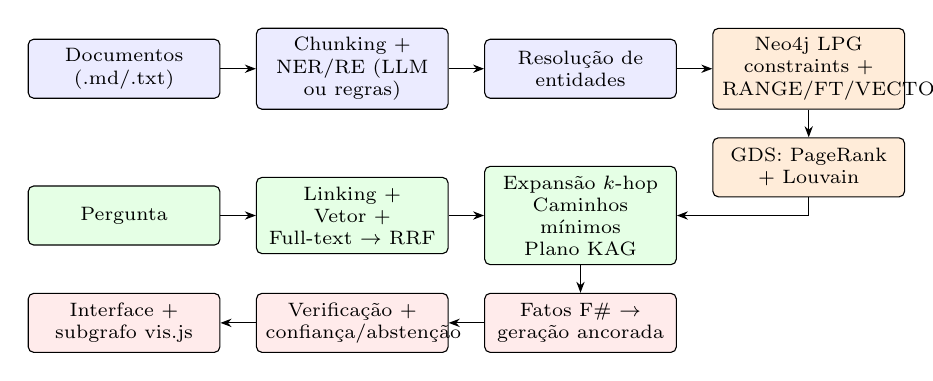
\begin{tikzpicture}[node distance=0.35cm and 0.45cm, font=\scriptsize,
  box/.style={draw, rounded corners=2pt, align=center, minimum height=0.75cm, text width=2.2cm, fill=#1},
  box/.default=white, >={Stealth[length=4pt]}]
\node[box=blue!8] (doc) {Documentos\\(.md/.txt)};
\node[box=blue!8, right=of doc] (ner) {Chunking +\\NER/RE (LLM\\ou regras)};
\node[box=blue!8, right=of ner] (er) {Resolução de\\entidades};
\node[box=orange!15, right=of er] (neo) {Neo4j LPG\\constraints +\\RANGE/FT/VECTOR};
\node[box=orange!15, below=of neo] (gds) {GDS: PageRank\\+ Louvain};
\node[box=green!10, below=1.1cm of doc] (q) {Pergunta};
\node[box=green!10, right=of q] (hyb) {Linking + Vetor +\\Full-text $\rightarrow$ RRF};
\node[box=green!10, right=of hyb] (trav) {Expansão $k$-hop\\Caminhos mínimos\\Plano KAG};
\node[box=red!8, below=of trav] (gen) {Fatos F\# $\rightarrow$\\geração ancorada};
\node[box=red!8, left=of gen] (ver) {Verificação +\\confiança/abstenção};
\node[box=red!8, left=of ver] (ui) {Interface +\\subgrafo vis.js};
\draw[->] (doc)--(ner); \draw[->] (ner)--(er); \draw[->] (er)--(neo); \draw[->] (neo)--(gds);
\draw[->] (q)--(hyb); \draw[->] (hyb)--(trav); \draw[->] (gds.south) |- (trav.east);
\draw[->] (trav)--(gen); \draw[->] (gen)--(ver); \draw[->] (ver)--(ui);
\end{tikzpicture}
\caption{Arquitetura: construção do grafo (azul), armazenamento e algoritmos (laranja), recuperação (verde) e geração com verificação (vermelho).}
\label{fig:arq}
\end{figure}

\subsection{Domínio, dados e modelagem LPG}

O domínio escolhido é a História da Computação, rico em relações encadeadas (orientador $\rightarrow$ instituição; criador $\rightarrow$ linguagem $\rightarrow$ laboratório). O corpus tem 15 documentos em português, um por personalidade ou tema.

O grafo possui duas camadas ligadas por \texttt{MENTIONS}. A camada lexical (\texttt{Document}, \texttt{Chunk}) guarda o texto e seus \textit{embeddings}; a camada de conhecimento usa um rótulo base \texttt{Entity} combinado a um rótulo de tipo (\texttt{Person}, \texttt{Organization}, \texttt{Location}, \texttt{Technology}, \texttt{Concept}, \texttt{Award}). O rótulo base permite um único índice vetorial e um único full-text sobre todas as entidades e uma constraint global de unicidade; o rótulo de tipo mantém as consultas seletivas. A ontologia define 15 tipos de relacionamento com domínio e alcance (ex.: \texttt{ADVISED}: Person$\rightarrow$Person; \texttt{DEVELOPED\_AT}: Technology$\rightarrow$Organization). Cada aresta de domínio guarda \texttt{sources} (ids dos \textit{chunks} que a afirmam), \texttt{year}, \texttt{confidence} e \texttt{mention\_count}: quando o mesmo fato aparece em dois documentos, o \texttt{MERGE} acumula as fontes em vez de duplicar a aresta.

O esquema é criado com 10 constraints de unicidade (\texttt{Entity.id}, uma por rótulo de tipo e as de \texttt{Document}, \texttt{Chunk} e \texttt{Community}), índices RANGE em nome, tipo, PageRank, comunidade, documento e no ano da relação \texttt{RECEIVED}, índices full-text sobre nomes/aliases e sobre o texto dos \textit{chunks} (analisador \texttt{brazilian}) e índices vetoriais de cosseno para \textit{chunks} e entidades:

\begin{lstlisting}[language=cypher]
CREATE CONSTRAINT entity_id IF NOT EXISTS FOR (e:Entity) REQUIRE e.id IS UNIQUE
CREATE FULLTEXT INDEX entity_fulltext IF NOT EXISTS FOR (e:Entity) ON EACH [e.name, e.aliases_text]
CREATE VECTOR INDEX chunk_embedding IF NOT EXISTS FOR (c:Chunk) ON c.embedding
  OPTIONS {indexConfig: {`vector.dimensions`: 384, `vector.similarity_function`: 'cosine'}}
\end{lstlisting}

\subsection{Pipeline Text-to-Graph}

Os documentos são divididos em \textit{chunks} por parágrafo, respeitando limites de sentença. Dois extratores compartilham a mesma interface. O \textbf{extrator LLM} recebe a descrição da ontologia e um exemplo, e devolve JSON com entidades e relações; a saída é validada: tipos fora do esquema são descartados (modo estrito) ou registrados (modo dinâmico), relações com direção invertida são corrigidas pela assinatura domínio/alcance e relações cujas entidades não foram declaradas são rejeitadas. O \textbf{extrator por regras}, usado no modo \textit{offline}, faz NER por dicionário com casamento do maior trecho --- o que distingue, por exemplo, ``Prêmio Turing'', ``Máquina de Turing'' e ``Turing'', e as duas cidades chamadas Cambridge --- e RE por padrões lexicais aplicados ao texto entre duas menções, com restrições de tipo. Três heurísticas evitaram os erros mais frequentes: usar apenas a pista mais próxima da segunda menção; ignorar o par quando o trecho após uma entidade intermediária começa com particípio (``a linguagem C foi influenciada pela linguagem B, \textit{criada por} Ken Thompson'' não gera \textit{Thompson criou C}); e ignorar adjuntos preposicionais da entidade intermediária (``fundou o W3C \textit{no} MIT'' não gera \textit{fundou o MIT}).

A \textbf{resolução de entidades} é feita em cascata, sempre restrita ao mesmo tipo: alias normalizado (sem acentos e pontuação), sobrenome único de pessoa, igualdade de tokens significativos, similaridade de Levenshtein acima de 0,90 --- com uma guarda que impede fundir nomes que diferem em tokens curtos ou números, como ``linguagem B'' e ``linguagem C'' --- e, opcionalmente, similaridade de \textit{embeddings}. Os ids são determinísticos (\texttt{person:alan\_turing}), o que torna a ingestão idempotente e incremental. O grafo resultante tem 99 entidades e 134 relações de domínio.

Após a ingestão, PageRank e Louvain são executados no Neo4j Graph Data Science (com \textit{fallback} em NetworkX quando o plugin não está disponível) e cada comunidade recebe um resumo, gerado por LLM ou por \textit{template}.

\subsection{Recuperação híbrida e multi-hop}

Dada uma pergunta, o sistema (1) recupera \textit{chunks} por busca vetorial; (2) liga menções da pergunta a entidades do grafo (\textit{entity linking}) e detecta nomes próprios que não existem no grafo; (3) consulta os índices vetorial e full-text de entidades e coleta as entidades mencionadas nos melhores \textit{chunks}; (4) funde essas quatro listas com RRF ($k=60$), dando prioridade às âncoras ligadas exatamente; (5) expande a vizinhança das âncoras com \texttt{[:REL*1..k]}, ordenando os caminhos por comprimento e PageRank; e (6) calcula \texttt{allShortestPaths} entre pares de âncoras. Cada aresta recuperada vira um fato numerado (F1, F2, \ldots), pontuado por origem (plano KAG $>$ caminho mínimo $>$ expansão), por coincidir com as relações citadas na pergunta e pela centralidade dos nós; os 30 melhores formam o contexto, junto com os \textit{chunks} de proveniência e os resumos das comunidades das âncoras.

\subsection{KAG: raciocínio por forma lógica}

No modo KAG, a pergunta é compilada em um plano com dois operadores. \texttt{chain} é uma sequência de passos \texttt{(origem)-[REL]->(variável)}, em que a origem é uma âncora ou uma variável anterior, com direção e tipo-alvo; uma variável atribuída por dois passos é a interseção dos resultados. \texttt{path} busca caminhos mínimos entre âncoras, filtrados pelo tipo da resposta e pelas relações da pergunta. Para ``Onde trabalhava o orientador de Alan Turing?'', o plano é \texttt{Alan Turing <-[ADVISED]- x1 -[WORKED\_AT]-> x2}.

O plano é produzido por um LLM, que recebe o esquema e as âncoras e responde em JSON validado, ou, sem LLM, por um planejador heurístico que associa pistas lexicais a relações, ordena os passos pela distância à âncora e decide a direção pela assinatura domínio/alcance da ontologia (para relações Pessoa$\rightarrow$Pessoa, pela posição da âncora em relação ao verbo). Em ambos os casos o LLM nunca escreve Cypher: cada passo é traduzido em um \textit{template} parametrizado cujos rótulos e tipos interpolados são verificados contra a ontologia. Após a execução, uma poda para trás remove valores intermediários que não levam à resposta, de modo que só os fatos efetivamente usados sejam citados. Complementarmente, quando há LLM e Neo4j, um módulo Text2Cypher gera consultas livres protegidas por validação estática (somente leitura, rótulos e tipos do esquema, \texttt{LIMIT} obrigatório), \texttt{EXPLAIN} prévio com uma tentativa de autocorreção e execução em transação de leitura.

\subsection{Geração ancorada e mitigação de alucinações}

A mitigação atua em três estágios. \textbf{Antes da geração}, o contexto contém apenas fatos numerados com fonte, caminhos e trechos; se a pergunta menciona uma entidade inexistente no grafo (premissa não verificável, como ``Prêmio Nobel'' de Dennis Ritchie), o sistema se abstém sem consultar o gerador. \textbf{Durante}, o \textit{prompt} exige uso exclusivo do contexto, uma citação por frase e uma frase padrão de abstenção, com temperatura zero; sem LLM, um gerador extrativo verbaliza os fatos do plano KAG. \textbf{Depois}, um verificador mede a cobertura de citações válidas por frase, a fração de entidades da resposta presentes no contexto recuperado e a ocorrência de nomes próprios que não existem nem no grafo nem nos trechos. A confiança final é
\begin{equation}
c = 0{,}45\,r + 0{,}30\,q + 0{,}25\,g,
\end{equation}
em que $r$ é a confiança da recuperação (âncoras ligadas, plano executado, fatos encontrados), $q$ a cobertura de citações e $g$ o aterramento de entidades, com penalidades multiplicativas para citações inválidas ($\times 0{,}7$) e entidades não aterradas ($\times 0{,}5$). Respostas com $c < 0{,}35$ são substituídas por abstenção.

\subsection{Interface e rastreabilidade}

A interface em Streamlit mostra a resposta com citações e o nível de confiança, e organiza a rastreabilidade em abas: o subgrafo interativo (vis-network), com âncoras, resposta e caminho do raciocínio destacados; a tabela de fatos com origem e \textit{chunks} de procedência; o plano KAG e sua execução passo a passo; todas as consultas Cypher executadas, com parâmetros e tempo; o relatório de verificação com o contexto exato enviado ao gerador; e os sinais de recuperação (âncoras, sementes RRF, \textit{chunks} e comunidades). Há ainda páginas de ingestão de novos documentos, exploração do grafo e avaliação. A Figura~\ref{fig:subgrafo} mostra o subgrafo de contexto de uma pergunta multi-hop.

\begin{figure}[ht]
\centering
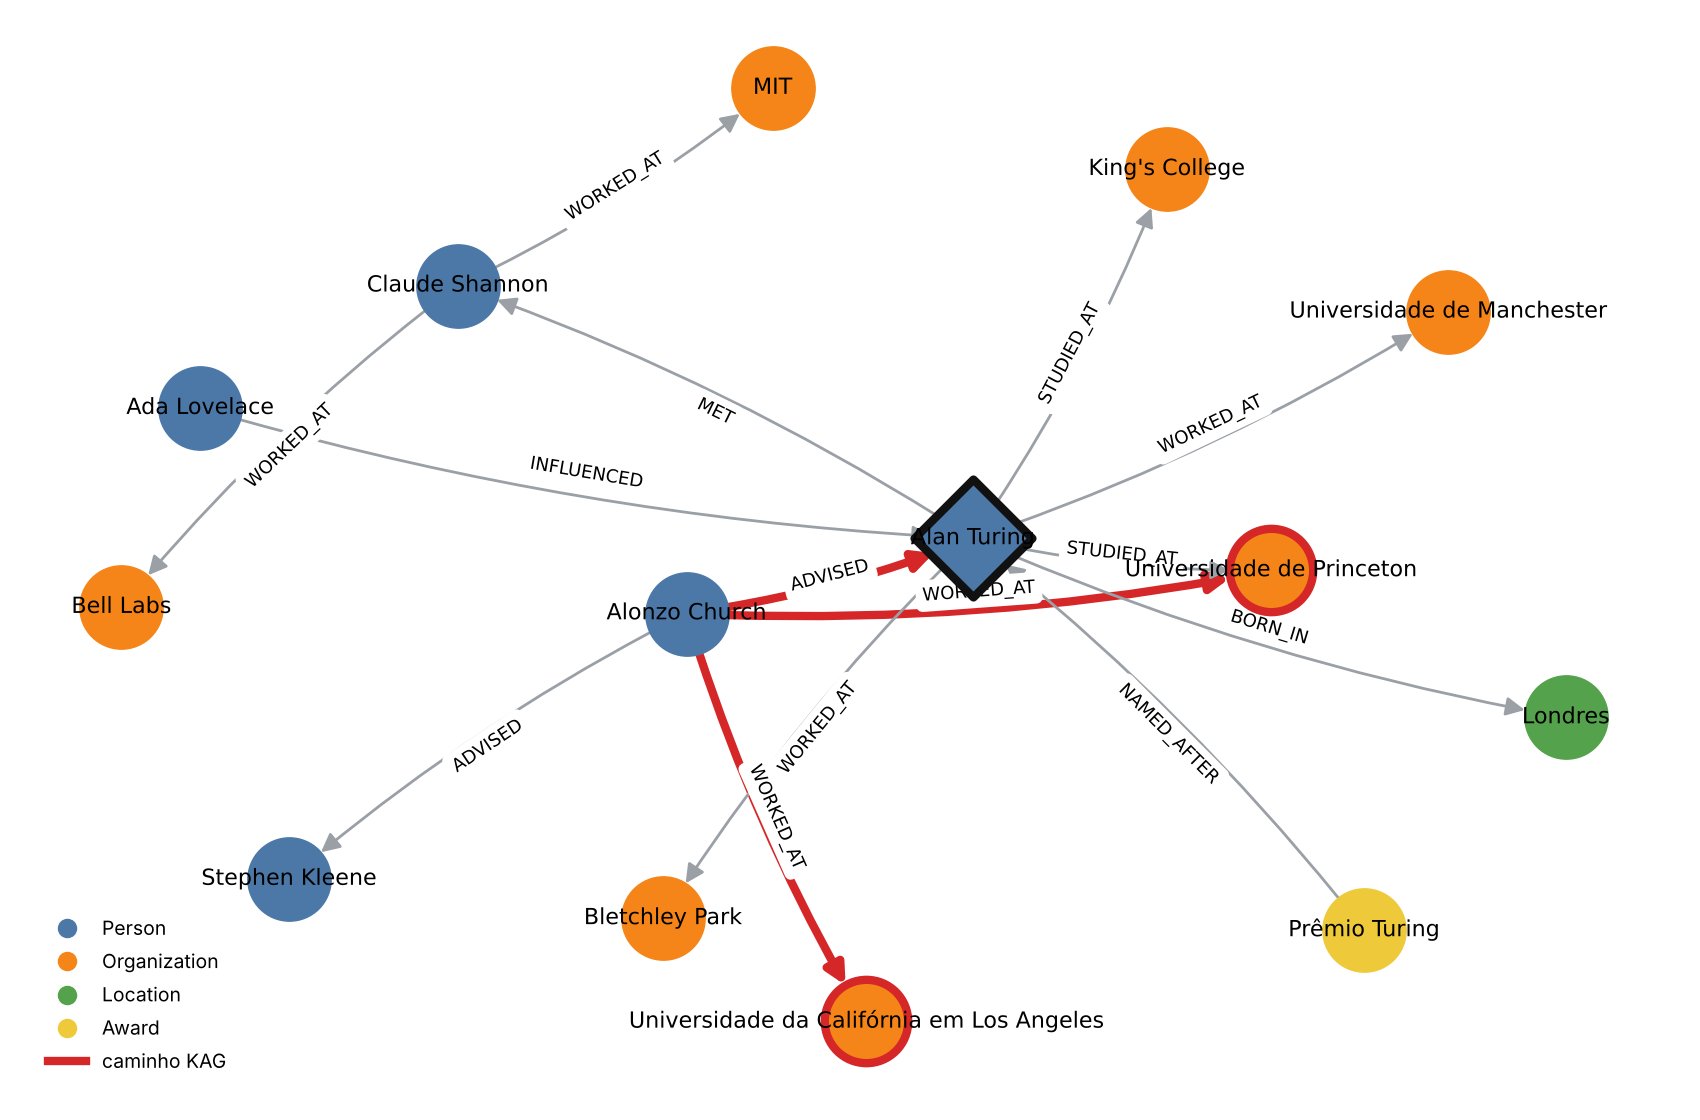
\includegraphics[width=0.88\textwidth]{figuras/subgrafo_turing.png}
\caption{Subgrafo de contexto para ``Onde trabalhava o orientador de Alan Turing?''. A âncora aparece como losango, as arestas do plano KAG em vermelho e as respostas com borda vermelha.}
\label{fig:subgrafo}
\end{figure}

% ======================================================================
\section{Avaliação Experimental}

\subsection{Configuração}

Comparamos três modos: \textbf{RAG vetorial} (somente \textit{chunks}), \textbf{GraphRAG} (recuperação híbrida, expansão, caminhos mínimos e comunidades) e \textbf{KAG} (GraphRAG + forma lógica). Todos os experimentos foram executados no modo \textit{offline}: extração por regras, \textit{embeddings} por \textit{feature hashing} de palavras e trigramas (384 dimensões) e gerador extrativo, o que os torna determinísticos e reprodutíveis com um único comando.

Usamos dois conjuntos de perguntas. O de \textbf{desenvolvimento} (21 perguntas: 7 de um salto, 10 multi-hop, 1 de caminho e 3 sem resposta no corpus) foi usado durante a construção do sistema, inclusive para ajustar o planejador heurístico, e por isso é otimista. O de \textbf{teste} (14 perguntas: 5, 6, 1 e 2, respectivamente) foi escrito depois, com outras formulações, e não foi usado para ajustes.

As métricas são: \textit{acurácia} (a resposta contém todas as entidades esperadas, ou o sistema se absteve quando não há resposta); \textit{precisão da resposta} (fração das entidades da linha de resposta que são esperadas); \textit{recall de contexto} (fração das entidades esperadas presentes no contexto entregue ao gerador, independente do gerador); \textit{abstenção correta}; e \textit{respostas não suportadas}, \textit{proxy} de alucinação que conta respostas dadas a perguntas sem resposta ou contendo entidades fora do contexto.

\subsection{Resultados}

\begin{table}[ht]
\centering
\caption{Resultados no conjunto de teste (14 perguntas, não usado no desenvolvimento).}
\label{tab:teste}
{\small\setlength{\tabcolsep}{4pt}\begin{tabular}{lcccccc}
\toprule
Modo & Acurácia & Multi-hop & Precisão & Recall ctx. & Abstenção & Não sup.$\downarrow$ \\
\midrule
RAG vetorial & 14\% & 0\% & 17\% & 88\% & 0\% & 14\% \\
GraphRAG híbrido & 57\% & 14\% & 46\% & 100\% & 100\% & 0\% \\
KAG (forma lógica) & \textbf{79\%} & \textbf{57\%} & \textbf{60\%} & 100\% & 100\% & \textbf{0\%} \\
\bottomrule
\end{tabular}}
\end{table}

\begin{table}[ht]
\centering
\caption{Resultados no conjunto de desenvolvimento (21 perguntas; otimista por ter guiado o desenvolvimento).}
\label{tab:dev}
{\small\setlength{\tabcolsep}{4pt}\begin{tabular}{lcccccc}
\toprule
Modo & Acurácia & Multi-hop & Precisão & Recall ctx. & Abstenção & Não sup.$\downarrow$ \\
\midrule
RAG vetorial & 24\% & 18\% & 20\% & 97\% & 0\% & 14\% \\
GraphRAG híbrido & 71\% & 46\% & 56\% & 100\% & 100\% & 0\% \\
KAG (forma lógica) & 100\% & 100\% & 82\% & 100\% & 100\% & 0\% \\
\bottomrule
\end{tabular}}
\end{table}

As Tabelas~\ref{tab:teste} e~\ref{tab:dev} mostram o mesmo padrão nos dois conjuntos. O resultado mais revelador é a distância entre recall de contexto e acurácia no RAG vetorial: em 88\% das perguntas de teste a informação necessária estava nos \textit{chunks} recuperados, mas a resposta só foi correta em 14\%. Recuperar trechos semelhantes à pergunta não basta quando a resposta exige compor fatos de documentos diferentes. O GraphRAG eleva o recall de contexto a 100\% e acerta todas as perguntas de um salto, mas, sem decompor a pergunta, ainda falha na maioria das multi-hop; o KAG, ao executar a cadeia de relações no grafo, chega a 57\% nelas no teste.

Quanto à alucinação, os dois modos com grafo se abstiveram em todas as perguntas sem resposta --- tanto as que pedem uma relação ausente (``Quem orientou o doutorado de Grace Hopper?'') quanto as com premissa falsa (``Em que ano Dennis Ritchie ganhou o Prêmio Nobel?'', ``Quem criou a linguagem Python?'') --- e não produziram nenhuma resposta não suportada. O baseline vetorial respondeu a todas com a frase mais similar do contexto. A latência média foi de 3~ms no modo vetorial e de 12--16~ms nos modos com grafo, no backend em memória.

\subsection{Análise de erros}

As três falhas do KAG no conjunto de teste e a baixa precisão de uma quarta pergunta indicam limitações concretas do planejador heurístico:
\begin{itemize}
  \item \textbf{Ambiguidade lexical} (``Quem criou a linguagem que foi influenciada pela linguagem B?''): a pista ``criou'' mapeia tanto \texttt{CREATED} quanto \texttt{DEVELOPED\_AT}; a partir de uma tecnologia, ambas são válidas, e o plano retornou o laboratório em vez da pessoa.
  \item \textbf{Salto implícito} (``Em que país nasceu Edsger Dijkstra?''): a pergunta pede um país, mas só o verbo ``nasceu'' aparece; falta o passo \texttt{LOCATED\_IN}, e a resposta parou na cidade (Roterdã).
  \item \textbf{Atalho no caminho mínimo} (``Quem trabalhou no MIT e criou a linguagem Lisp?''): a aresta direta \texttt{Lisp-DEVELOPED\_AT->MIT} torna o caminho mínimo de comprimento 1, sem nó intermediário do tipo Pessoa. Um plano de interseção (\texttt{MIT<-WORKED\_AT-x}, \texttt{Lisp<-CREATED-x}) resolveria o caso.
  \item \textbf{Restrição por atributo} (``Quem recebeu o Prêmio Turing em 1974?''): a resposta correta foi incluída, mas junto com todos os laureados, pois o vocabulário de operadores não tem filtro por propriedade (precisão de 1/7).
\end{itemize}
Os quatro casos são cobertos pelo formato de plano usado pelo planejador LLM (interseção e tipos-alvo explícitos), e o terceiro e o quarto sugerem extensões diretas do vocabulário de operadores.

% ======================================================================
\section{Discussão e Limitações}

Os números indicam tendências, não significância estatística: o corpus e os conjuntos de perguntas são pequenos. O modo \textit{offline} penaliza principalmente o baseline vetorial, cujo gerador extrativo não consegue compor fatos de duas frases; com um LLM, espera-se que a distância diminua nas perguntas de um salto, mas o recall de contexto e a ausência de raciocínio explícito continuam a favorecer os modos com grafo nas perguntas multi-hop. O extrator por regras depende do dicionário de entidades para reconhecer nomes novos (o cabeçalho \texttt{subject} do documento ameniza isso), e os \textit{embeddings} por \textit{hashing} capturam sobreposição lexical, não sinonímia. Por fim, a regra de abstenção por nome próprio desconhecido é conservadora: perguntas que citam eventos não modelados (por exemplo, ``Segunda Guerra Mundial'') também levam à abstenção.

% ======================================================================
\section{Conclusão}

Apresentamos um sistema GraphRAG/KAG completo sobre Neo4j que cobre extração de entidades e relações com resolução de entidades, modelagem LPG com constraints e índices RANGE, full-text e vetoriais, recuperação híbrida com fusão RRF, travessia multi-hop enriquecida por PageRank e comunidades, raciocínio por forma lógica com Cypher seguro e uma interface que expõe o subgrafo, os fatos, o plano, as consultas e a confiança de cada resposta. No conjunto de teste, a decomposição lógica foi o fator decisivo para perguntas multi-hop, e os mecanismos de aterramento eliminaram as respostas não suportadas. Como trabalhos futuros, propomos operadores de filtro por atributo e de agregação, avaliação com LLMs locais e comerciais em conjuntos maiores e comunidades hierárquicas com Leiden para perguntas globais. O código, os dados e os scripts de avaliação estão no repositório do projeto.

\bibliographystyle{apalike}
\bibliography{refs}

\end{document}
